\documentclass[10pt,conference,compsocconf]{IEEEtran}

\usepackage{hyperref}
\usepackage{graphicx}	% For figure environment
\usepackage{textcomp}
\usepackage[english]{babel} % English language/hyphenation
\usepackage{amsmath,amsfonts,amsthm} % Math packages
\usepackage{algorithm} 
\usepackage{bbm}
\usepackage{algorithmic} 
\usepackage{multirow}
\usepackage{booktabs}
\usepackage{graphicx}
\usepackage{svg}
\usepackage{bm}
\usepackage{hyperref}
\usepackage{subcaption}
\usepackage{float}

\begin{document}
\title{Evaluating the quality of videos through machine learning}

\author{
  FENG Wentao, ZHUANG Ying, WANG Yunbei\\
  \textit{Science et Techniques de l'Ingénieur, EPFL, Switzerland}
}

\maketitle

\begin{abstract}
  This essay tries to build a machine learning model in order to evaluate the quality of videos or images. Two models are built, and their results are compared.
\end{abstract}

\section{Introduction}
The overall goal of our project is to discover a method to predict the quality of a compressed omnidirectional image or video quality.  Some open data sets provide subjective scores which are usually integer values on the range from 1(poor) to 5(excellent) or from 0 to 100. Moreover, from the tutor, we get some features of the compressed content. The idea is to train regression models based on the part of or all of the features to evaluate the quality of videos.

\section{Feature description}
There are two kinds for our feature: the full reference metrics and no reference metrics. 
\subsection{No reference metrics}
\label{nr_metrics}
For the no reference metrics\footnote{Video Quality Indicators, \url{http://vq.kt.agh.edu.pl/metrics.html}}, they can be directly extracted from each frame of the video and their detailed information is listed as following:
\begin{description}
\item[Commercial Black] \ \\
  $min = 0$, $max = 1$, no distortion exists if value equals to 0 and greater value means greater distortion.
\item[Blockiness] \ \\
  $min = 0$, $max = 3570$, no distortion exists if value ranges from 0.9 to 1.01 and greater value means less distortion.
\item[Block Loss] \ \\
  $min = 0$, $max = 100 - 200$, no distortion exists if value ranges from 0 to 5 and greater value means more distortion.
\item[Blur] \ \\
  $min = 0$, $max \approx 70$, no distortion exists if value ranges from 0 to 5 and greater value means greater distortion.
\item[Contrast] \ \\
  $min = 0$, $max \approx 120$, no distortion exists if value ranges from 45 to 55 and greater value means higher contrast. This metric is not directly relevant to the distortion.
\item[Exposure] \ \\
  $min = 0$, $max = 255$, no distortion exists if value ranges from 115 to 125 and greater value means longer exposure time. This metric is not directly relevant to the distortion.
\item[Flickering] \ \\
  $min = 0$, $max = 8$, the typical value for time window with 8 frames is 0.125 and greater value means higher distortion.
\item[Freezing] \ \\
  $min = 0$, $max = 1$, no distortion exists if value equals to 0 and greater value means greater distortion. This metric is coupled with the results of Temporal Activity.
\item[Interlacing] \ \\
  $min = 0$, $max = 1$, no distortion exists if value equals to 0 and greater value means greater distortion.
\item[Letter-boxing] \ \\
  $min = 0$, $max = 1$, no distortion exists if value equals to 0 and greater value means greater distortion.
\item[Noise] \ \\
  $min = 0$, $max = 1$, no distortion exists if value ranges from 0 to 3.5 and greater value means greater distortion.
\item[Pillar-boxing] \ \\
  $min = 0$, $max = 1$, no distortion exists if value equals to 0 and greater value means greater distortion.
\item[Slicing] \ \\
  $min \approx 0$, $max = 1$, this metric does not work properly.
\item[Spatial Activity] \ \\
  $min = 0$, $max \approx 270$, no distortion exists if value ranges from 0 to 60 and greater value means greater spatial activity.
\item[Temporal Activity] \ \\
  $min = 0$, $max = 255$, no distortion exists if value ranges from 0 to 20 and greater value means greater temporal activity.
\end{description}
\begin{table*}[htbp]
  \centering
  \begin{tabular}[c]{|l||l|l|l|l|l|}
    \hline
    Feature & Slice & Blackout & Freezing & Letterbox & Pillarbox\\
    \hline
    min & 1.01 & 0 & 0 & 0 & 0\\
    25\% & 6.20 & 0 & 0 & 0 & 0\\
    50\% & 10.31 & 0 & 0 & 0 & 0\\
    75\% & 23.34 & 0 & 0 & 0 & 0\\
    max & inf & 0 & 0 & 0.23 & 0.10\\
    \hline
  \end{tabular}
  \caption{Invalid features}
  \label{drop_feature}
\end{table*}
\subsection{Full reference metrics}
Full reference metrics provide a relative assessment to the compressed video. These metrics are calculated by setting the original video as a reference. In this project, we believe all full metrics are useful and valid and take all the metrics into account when we build the model.


\section{Data processing}
\subsection{Validity verification}
To filter invalid no reference metrics, we calculate some common statistic characters for each metric. Then, we can distinguish weird features that are listed in table \ref{drop_feature}. The \texttt{Slice} is invalid as we mentioned in \ref{nr_metrics}. For the \texttt{Blackout} and \texttt{Freezing}, all the frames are the same in these two metrics. So, we remove them naturally. Only few videos have distortion in \texttt{Letterbox} and \texttt{Pillarbox}. Therefore, these two are relinquished. All other features are in reasonable range and completely recorded and thus all of them are kept.
\subsection{Pooling method}
Each video has many frames, and we have features for each frame. However, for one individual video, we only need one value for each feature. So, we need to collapse series of frame features to one feature for the whole video sequence. The temporal pooling method we used is called Minkowski summation and the Minkowski exponent $p = 4$. The pooling formula is
\begin{equation}
(\frac{1}{n}\sum_{frame = 1}^{n} frame^{p})^{\frac{1}{p}}
\end{equation}


\section{Measurement method}
In order to evaluate the quality of regression, we introduce three measurement methods to make evaluation comprehensively.
\subsection{Root Mean Square Error}
Root Mean Square Error(RMSE) is the standard deviation of the prediction errors. It calculates the residuals that are a measure of how far the original data points from the predicted data points are. Moreover, RMSE is a measure of how spread out these residuals is. In other words, small RMSE means the predicted data concentrate around the original curve, which implies the prediction is good. The equation for RMSE is
\begin{equation}
RMSE = [\frac{1}{N}\sum_{i=1}^{N}(y_{pred} - y_{true})^2]^{\frac{1}{2}}    
\end{equation}

\subsection{Linear Correlation Coefficient}
Linear Correlation Coefficient(LCC) is also called the Pearson correlation coefficient, which is a measure of the linear correlation between two variables $X$ and $Y$. The range of LLC is from -1 to 1. If LCC equals to -1(1), then those two variables have a negative(positive) linear relationship. 0 means completely no linear relationship. The equation for LCC is
\begin{equation}
    \rho_{X, Y} = \frac{cov(X, Y)}{\sigma_X \sigma_Y }
\end{equation}
where $cov$ is the covariance, $\sigma_{X(Y)}$ is the standard deviation of $X(Y)$.

\subsection{Spearman's Rank Correlation Coefficient}
Spearman's rank correlation coefficient(SRCC) mainly assesses how well the relationship between two variables can be described using a monotonic function. The equation for SRCC is
\begin{equation}
    r_S = \rho_{rg_X,r_X} = \frac{cov(rg_X, rg_Y)}{\sigma_{rg_X} \sigma_{rg_Y}}
\end{equation}
where $rg$ denotes ranks, $\rho$ denotes LCC, $cov$ denotes covariance and $\sigma$ denotes standard deviation.

For the regression problem, small RMSE guarantees our fitted curve is close to the original one. Meanwhile, large LCC and SRCC guarantee those two have a similar trend. Therefore, we utilize these three metrics as the measurements. Moreover, RMSE is the primary measurement in our model, as we want to predict the score as close to the real one as possible.

\section{Random forest model}
Random Forest is a flexible, easy to use machine learning algorithm. The main idea of it is generating many random decision trees and finding a tree that fits the data well. The randomness helps it get a good result even without hyperparameter tuning. We choose it as our first model and compare it with Support Vector Regression later. Also, some aspects are keys to the performance of our random forest model.

\begin{figure*}[htbp]
\centering
\includegraphics[width = \linewidth]{comparasion_predit_real_rf.pdf}
\caption{Random Forest - Prediction result on the test set}
\label{result_rf}
\end{figure*}

\subsection{Group cross validation}
As we learned in the lecture, cross-validation(CV) is a simple technique to avoid overfitting in regression. The most common CV method is K-fold. Specifically, we equally split data set into $K$ folds, and $K-1$ folds are training set, and one fold is test set. Hence, for each dataset, we can train $K$ times and select the model that works well both on the training set and the test set. However, for our dataset, we need to do some additional limitation on the split of train data and test data. Observing the names of videos, we find that each original video is compressed to three extents, namely, high compression ratio, medium compression ratio and low compression ratio. The compression ratio does not change much on the features. In other words, these three compressed videos are close in multi-dimension space. Therefore, we should group them in style in the table \ref{group_video} and thus avoid separating them into two sets. 
\begin{table}[h]
  \centering
  \begin{tabular}[c]{|l|l|}
    \hline
    Group 1 \\
    \hline
    G10BoatInPark\_ERP\_4096x2048\_fps30\_qp27\_14547k\\
    G10BoatInPark\_ERP\_4096x2048\_fps30\_qp37\_3270k\\
    G10BoatInPark\_ERP\_4096x2048\_fps30\_qp42\_1507k \\
    \hline
    Group 2  \\
    \hline
    G10BodybuildingWorkout\_ERP\_7680x3840\_fps29.97\_qp27\_6105k  \\
    G10BodybuildingWorkout\_ERP\_7680x3840\_fps29.97\_qp37\_913k  \\
    G10BodybuildingWorkout\_ERP\_7680x3840\_fps29.97\_qp42\_697k \\
    \hline
  \end{tabular}
  \caption{Grouped videos}
  \label{group_video}
\end{table}

\subsection{Hyper-parameter tuning by grid search}
Grid Search is a powerful tool to find the best hyper-parameters. Since hyper-parameter tuning relies more on experimental results than theory, it is necessary to try as many times as possible. We set the pool for each parameter and generate parameters gird through listing all possible combination. For each combination of parameters, we build a model and implement CV and select the parameter that predicts the most accurate result on the test dataset. The number of trees is a critical parameter for the random forest. The more trees are generated, more possible to find a good model. However, increasing the number of trees can increase the computing time especially when we use grid search. Normally, there are thousands of combination of parameters in a grid, and the folds of CV is 8. So, it is common that each grid search will build 1 million decision tree. It is very intractable to do grid search just once, since it may take one day to finish searching. For our case, we have implemented three grid search, and they take 7 minutes. We also try to do grid search once, but it fails to complete with one night.

\subsection{Finding best training set}
One of the major obstacles is that the dataset is incomplete. After filtering the unlabelled samples, only 177 samples remain, which means outliers can make significant effects on the accuracy of our model. After tuning the hyper-parameter, we modify CV to pick 80\% of samples randomly as subsets. Instead of training on the whole training set, we build the model on the subset. From statistic theory, if the number of the pick is big enough, we can finally find the best training set that reduces the influence of outliers.

\subsection{Results}
After three times of hyper-parameter grid search and discovering the best train set, we get a random forest that fits our case well. The measurement for this model is in table \ref{best_rf}.
\begin{table}[h]
  \centering
  \begin{tabular}[c]{|l||l|l|}
    \hline
    Measurement method & Score on train set & Score on test set\\
    \hline
    RMSE & 4.59 & 4.47 \\
    LCC & 0.93 & 0.91 \\
    SROCC & 0.94 & 0.90  \\
    \hline
  \end{tabular}
  \caption{The score of our best Random Forest model}
  \label{best_rf}
\end{table}
The RMSE on the training set and test set are both the lowest among all models. The LCC and SROCC are the closest to 1(entirely positive linear relationship). Moreover, the gap between measurement on the training dataset and test dataset is narrow, which means overfitting may not exist in our regression. The comparison between predicted score and original score on the test set is in figure \ref{result_rf}.


\begin{figure*}[htbp]
\centering
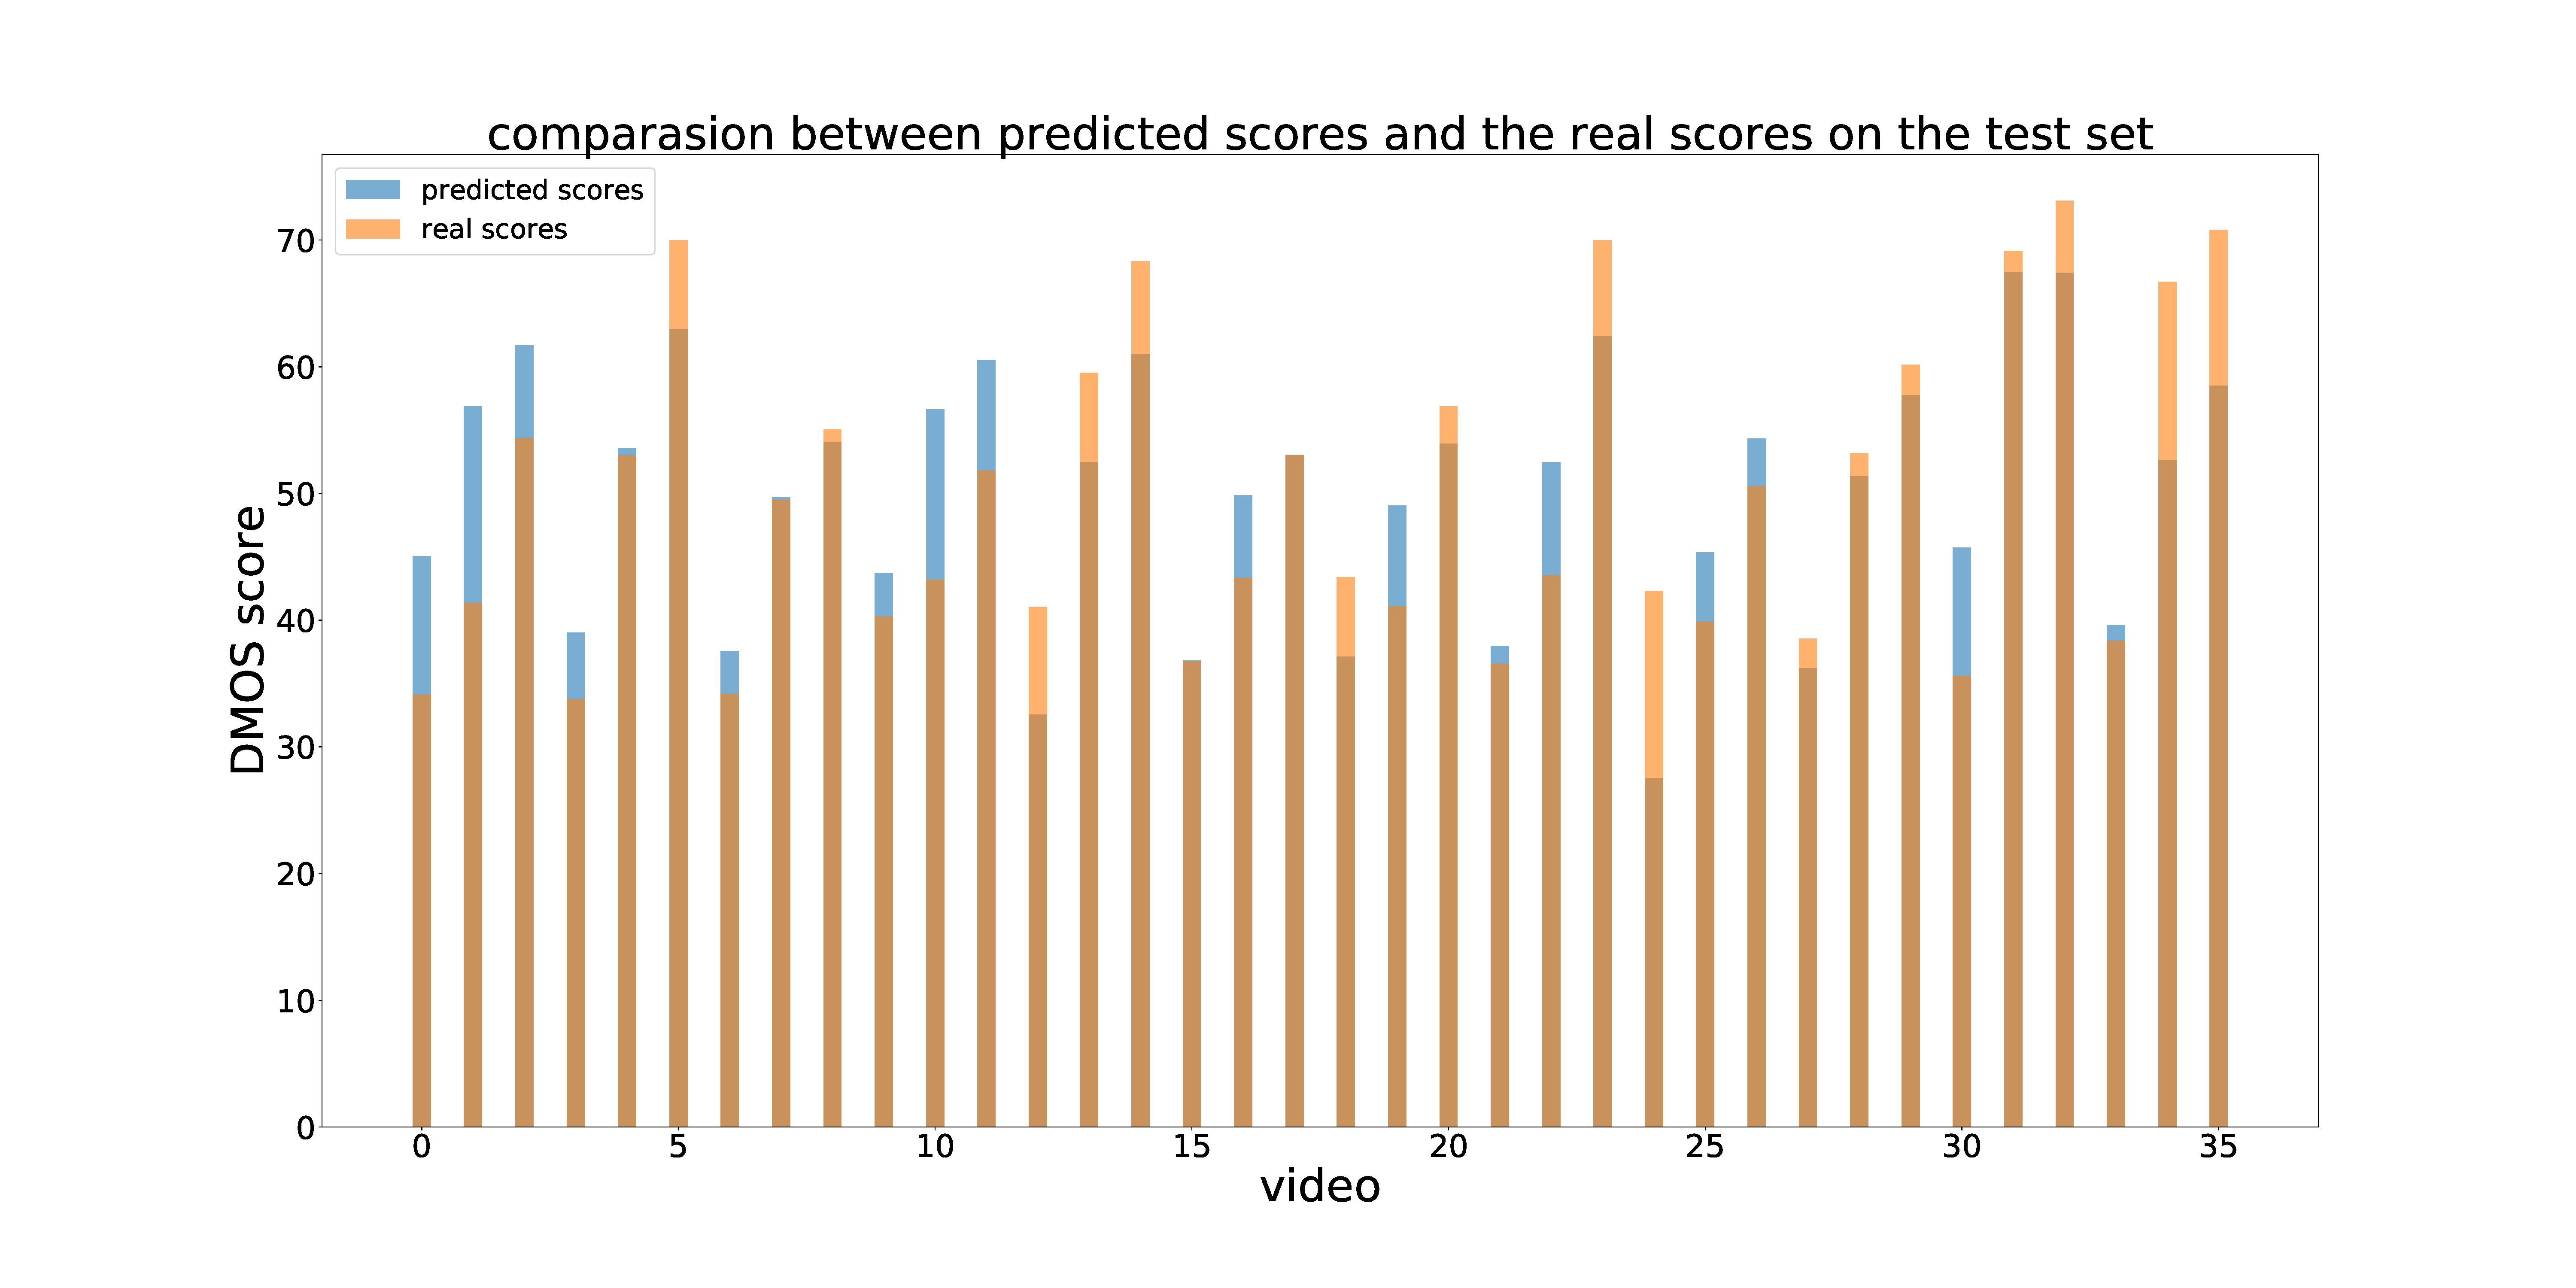
\includegraphics[width = \linewidth]{comparasion_predit_real.pdf}
\caption{Support Vector Regression - Prediction result on the test set}
\label{result_svr}
\end{figure*}

\section{Support vector regression model}
We also use the Support Vector Machine(SVM) method to solve our problem. This algorithm is widely used for data classification and regression analysis. In our case, we use DMOS values as the scores for videos, which are float numbers between 0 and 100. So instead of doing data classification, we use the SVM method to build the regression model. As we already performed feature processing, we will directly pass to hyperparameter tuning for our SVR model. First, we need to find the best kernel that describes our data whether it is linear, radial basis function (RBF), polynomial or sigmoid. Before tuning this parameter, we first perform a principal component analysis (PCA) in order to have a hint on how to choose the kernel. We reduce the dimension of the feature to 1 and visualize the data in a 2-D plot. The figure is shown in figure \ref{pca}:
\begin{figure}[h]
\centering
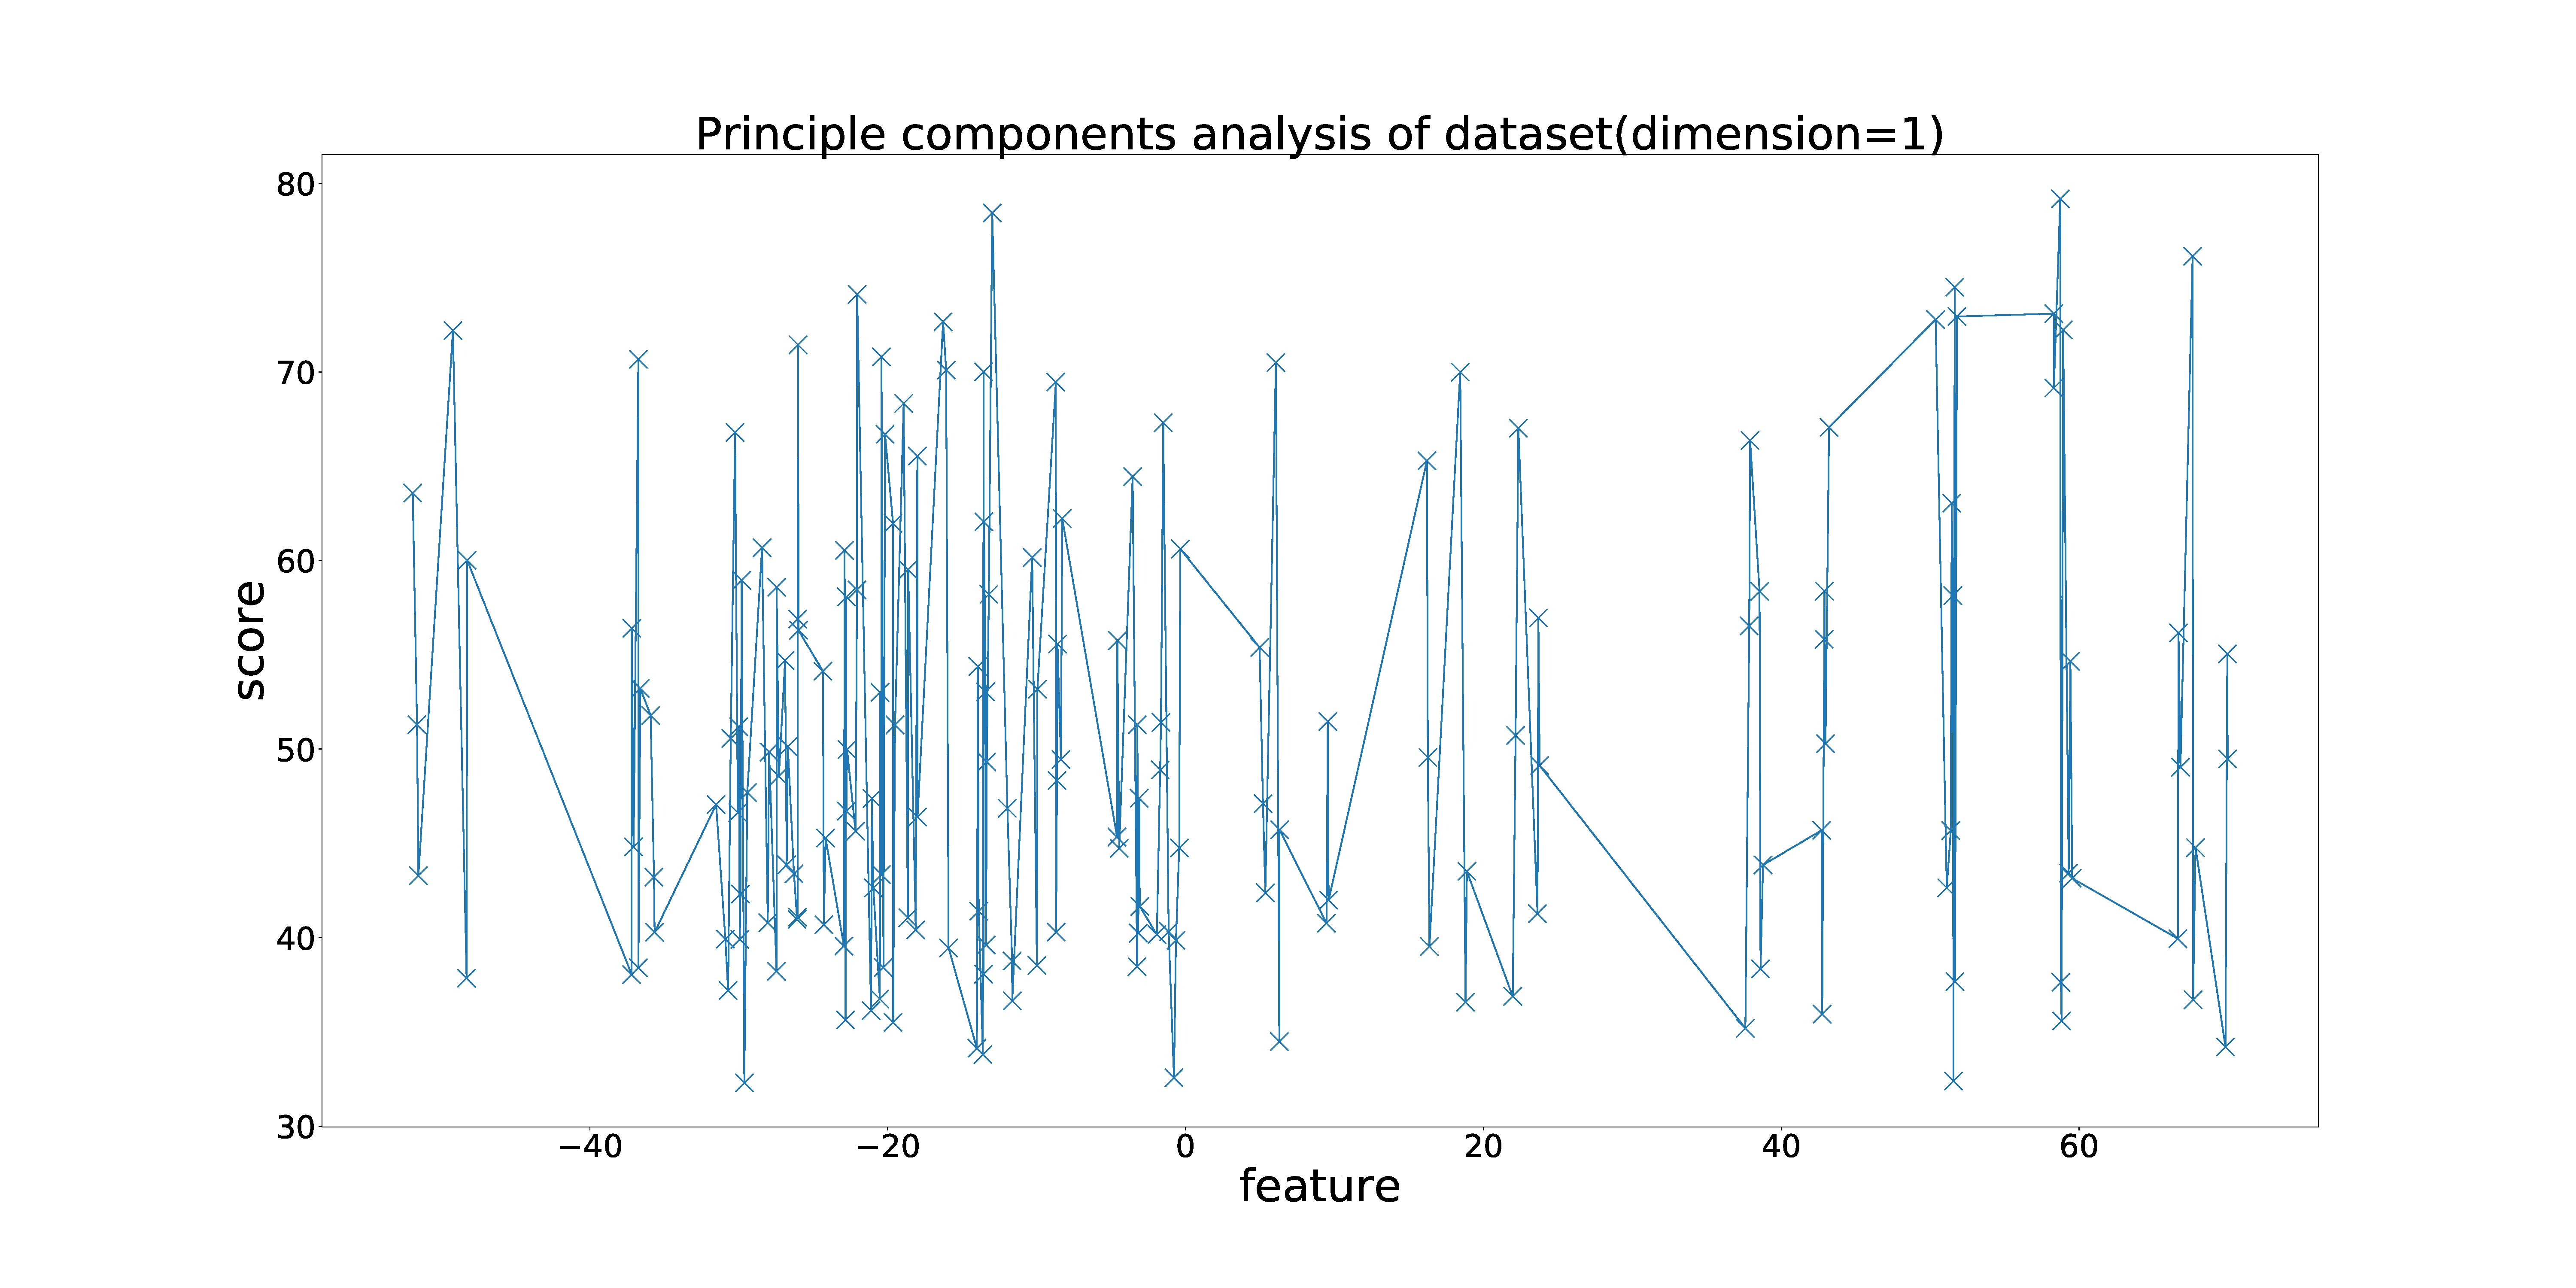
\includegraphics[trim = {2 0 2 0}, clip, width = \linewidth]{pca.pdf}
\caption{Feature and score represented in low dimension space}
\label{pca}
\end{figure}
\par Based on the observation, we find that the linear kernel is not suitable in our case. Moreover, because all the value of our output is finite and positive, so it is not very meaningful to use the sigmoid kernel. In consequence, we tune this parameter between the option RBF and polynomial. Another parameter significant is the penalty value of the error term C. This value should be bigger enough to avoid underfitting yet not too large otherwise the model might be overfitted. So we choose to tune this value inside the interval from 1 to 100. The value of Epsilon will also affect the accuracy of the model; it defines a margin of tolerance where the errors are not penalized. Its default value is 0.1, so we will perform the grid research between 0.05 and 0.3. This value could not be too larger otherwise the model will be over-fitted. Then for the RBF kernel, we have to tune its parameter gamma which is the inverse of the standard deviation of the Gaussian function. If gamma is too large, the variance of the Gaussian function becomes very small. Then our model only works on the samples that near the support vector, then it might be overfitted. Theoretically, the value of gamma should be small in order to have a better performance. So we try to find the best gamma among the value ‘0’,’0.01’,’auto’ and ’scale’ where ‘auto’ is equal to $\frac{1}{\text{n\_features}}$ and ‘scale’ is equal to $\frac{1}{(\text{n\_feature} * \sigma_X)}$. Then we perform grid search over the selected parameters based on the scores given by the RMSE method.
\par We use this model to do cross-validation over our dataset. The prediction score for our final-selected model over the training set and the test set is shown in table \ref{best_svr} and the predicted data on test set is in \ref{result_svr}.
\begin{table}[h]
  \centering
  \begin{tabular}[c]{|l||l|l|}
    \hline
    Measurement method & Score on train set & Score on test set\\
    \hline
    RMSE & 3.77 & 5.92 \\
    LCC & 0.95 & 0.84 \\
    SROCC & 0.96 & 0.89  \\
    \hline
  \end{tabular}
  \caption{The score of our best SVR model}
  \label{best_svr}
\end{table}

\section*{Acknowledgements}
The authors appreciate Azevedo Roberto in LTS4 for his careful tutoring and kindly help in the past 30 days, and scikit-learn\cite{scikit-learn} for providing many excellent modules.

\bibliographystyle{ieeetr}
\bibliography{refer}

\end{document}
